\section{Results}\label{sec:results}

Table~\ref{tab:model_selection} summarizes the pre-policy model-selection stage together with the naive benchmarks. The best average validation performance is obtained by LightGBM with a 6-step window, which reaches a mean MAE of 17.90 across the valid district-pollutant combinations. Among the learned models, LightGBM with a 24-step window is the second-best configuration at 20.60. The strongest naive comparator is the same-hour previous-day forecast at 20.52, while one-hour persistence is much weaker at 31.74. The stacked multivariate LSTM remains clearly weaker than LightGBM on average, and Ridge produces the largest post-policy gaps but also by far the worst pre-policy MAE. In other words, the most optimistic post-policy summaries are not attached to the most credible predictive baseline.

\begin{table}[htbp]
\centering
\caption{Pre-policy model-selection summary with learned models and naive baselines; post-policy PIP is shown only as a secondary reference}
\label{tab:model_selection}
\begin{tabular}{@{}lrrrr@{}}
\toprule
Model & Window & Mean MAE & Median MAE & Mean post PIP (\%) \\
\midrule
LightGBM & 6  & 17.90 & 13.36 & 70.18 \\
Seasonal naive & 24 & 20.52 & 16.88 & 68.85 \\
LightGBM & 24 & 20.60 & 15.58 & 73.24 \\
LSTM     & 6  & 24.02 & 14.32 & 18.97 \\
LSTM     & 24 & 24.12 & 14.52 & 17.88 \\
Persistence & 1  & 31.74 & 24.70 & 91.72 \\
Ridge    & 6  & 36.16 & 32.82 & 84.13 \\
Ridge    & 24 & 36.43 & 32.82 & 92.35 \\
\bottomrule
\end{tabular}
\end{table}

The naive baselines sharpen two points. First, the preferred LightGBM $w=6$ model improves on the strongest naive comparator by 2.62 MAE points, so the selected specification is not merely reproducing a simple daily seasonal heuristic. Second, the persistence forecast attains the largest mean post-policy PIP despite poor pre-policy fit, reinforcing why PIP should not be interpreted without a credible predictive baseline.

A supplementary rolling-origin check within 2021 keeps LightGBM as the preferred family and shows that the exact short-range window is not unique. Over three 30-day folds, LightGBM attains mean MAE values of 13.28 for $w=6$, 13.04 for $w=12$, and 13.62 for $w=24$, all better than the seasonal-naive benchmark at 14.74. The manuscript nevertheless retains $w=6$ as the principal specification because model selection is fixed exclusively by the pre-declared main split, where $w=6$ clearly outperforms the supplementary $w=12$ sensitivity (17.90 vs.\ 21.02 mean MAE). The rolling-origin exercise is used only to assess family-level stability and short-window stability, not to reopen model selection after seeing the main result.

The preferred specification is therefore the full-feature LightGBM model with window $w=6$. Table~\ref{tab:ablation_summary} summarizes the post-policy behavior of that specification under the main ablations. The full model yields a mean PIP of 70.18\%, a mean residual of 4.32, and a median residual of 4.93. Removing traffic leaves the aggregate signal almost unchanged, whereas removing meteorological variables lowers the mean PIP to 65.29\% and roughly halves the mean residual. The no-IQR run preserves the average PIP but worsens pre-policy MAE and increases the mean residual, which suggests that the outlier treatment affects magnitude more than direction. The no-traffic ablation attains a slightly smaller MAE (17.46 vs.\ 17.90), but the ablations are used as diagnostics rather than as a second model-selection stage, and the full model is retained because it preserves a substantively relevant mobility covariate even when its incremental predictive contribution is limited in this panel.

\begin{table}[htbp]
\centering
\caption{Post-policy summary for the preferred LightGBM $w=6$ specification and its minimal ablations}
\label{tab:ablation_summary}
\begin{tabular}{@{}lrrrr@{}}
\toprule
Variant & Mean MAE & Mean PIP (\%) & Mean residual & Median residual \\
\midrule
Full model & 17.90 & 70.18 & 4.32 & 4.93 \\
No traffic & 17.46 & 70.08 & 4.55 & 4.79 \\
No weather & 18.56 & 65.29 & 2.04 & 4.39 \\
No IQR     & 19.81 & 70.44 & 6.16 & 3.83 \\
\bottomrule
\end{tabular}
\end{table}

Uncertainty in the preferred post-policy summaries is modest at the aggregate level. A day-block bootstrap with 500 repetitions yields a 95\% interval of [69.32, 71.15] for mean PIP, [3.71, 5.01] for the mean residual, and [4.43, 5.34] for the median residual. These intervals remain on the positive side of zero for the residual-based summaries, so the aggregate signal is not driven by a small set of isolated hours.

Figures~\ref{fig:placebo} and \ref{fig:tradeoff} provide complementary diagnostics on temporal specificity and the fit-gap trade-off. Figure~\ref{fig:placebo} shows a fixed 60-day placebo exercise for the preferred LightGBM $w=6$ model. The January 2022 boundary yields larger positive gaps than the late-2021 placebo cuts: mean residual 8.96 and mean PIP 75.12\% against 6.77 and 73.54\% for October 2021, and 4.98 and 71.84\% for November 2021. The placebo contrast is supportive but not dispositive. Figure~\ref{fig:tradeoff} shows the trade-off between pre-policy fit and post-policy gap. The most spectacular gaps belong to weak baselines such as Ridge and persistence, whereas LightGBM offers the strongest predictive credibility with a still-positive aggregate deviation.

A direct one-step sensitivity with observed histories provides a more homogeneous comparison across model families. Under that sensitivity, LightGBM still has the best predictive ranking by MAE (9.28 for $w=6$ against 12.33 for Ridge and 24.02 for LSTM), but the mean post residual is -1.40. The reason is substantive rather than contradictory: once treated post-policy lags are inserted into the forecast window, the model is no longer estimating continuation of the untreated pre-policy regime. It is answering a different one-step prediction question. The direct sensitivity therefore strengthens the model-ranking argument, but not the no-change counterfactual itself.

At the district-pollutant level, the pattern remains positive in many cells but not uniformly so. Figure~\ref{fig:heatmap} shows the mean residuals for the preferred specification. PM$_{10}$ is the strongest and most consistent positive signal, especially in Villa de Vallecas, where the mean residual reaches 18.42 and PIP rises to 87.56\%. By contrast, NO is the least stable pollutant: its mean residual is slightly negative in all three districts even though PIP remains above 65\%, which illustrates why PIP alone is not sufficient to characterize the post-policy behavior. PM$_{2.5}$ is not reported for Villa de Vallecas because the retained station does not provide valid measurements for that pollutant in the final panel.

The traffic ablation needs a similarly local reading. Its aggregate effect is small, but not identically zero. Removing the district traffic proxy changes the Tetuan NO$_2$ mean residual by 2.74 and its PIP by 3.24 points. The available traffic variable is therefore not inert, but it is too coarse to support a strong mechanism claim.

\begin{figure}[htbp]
\centering
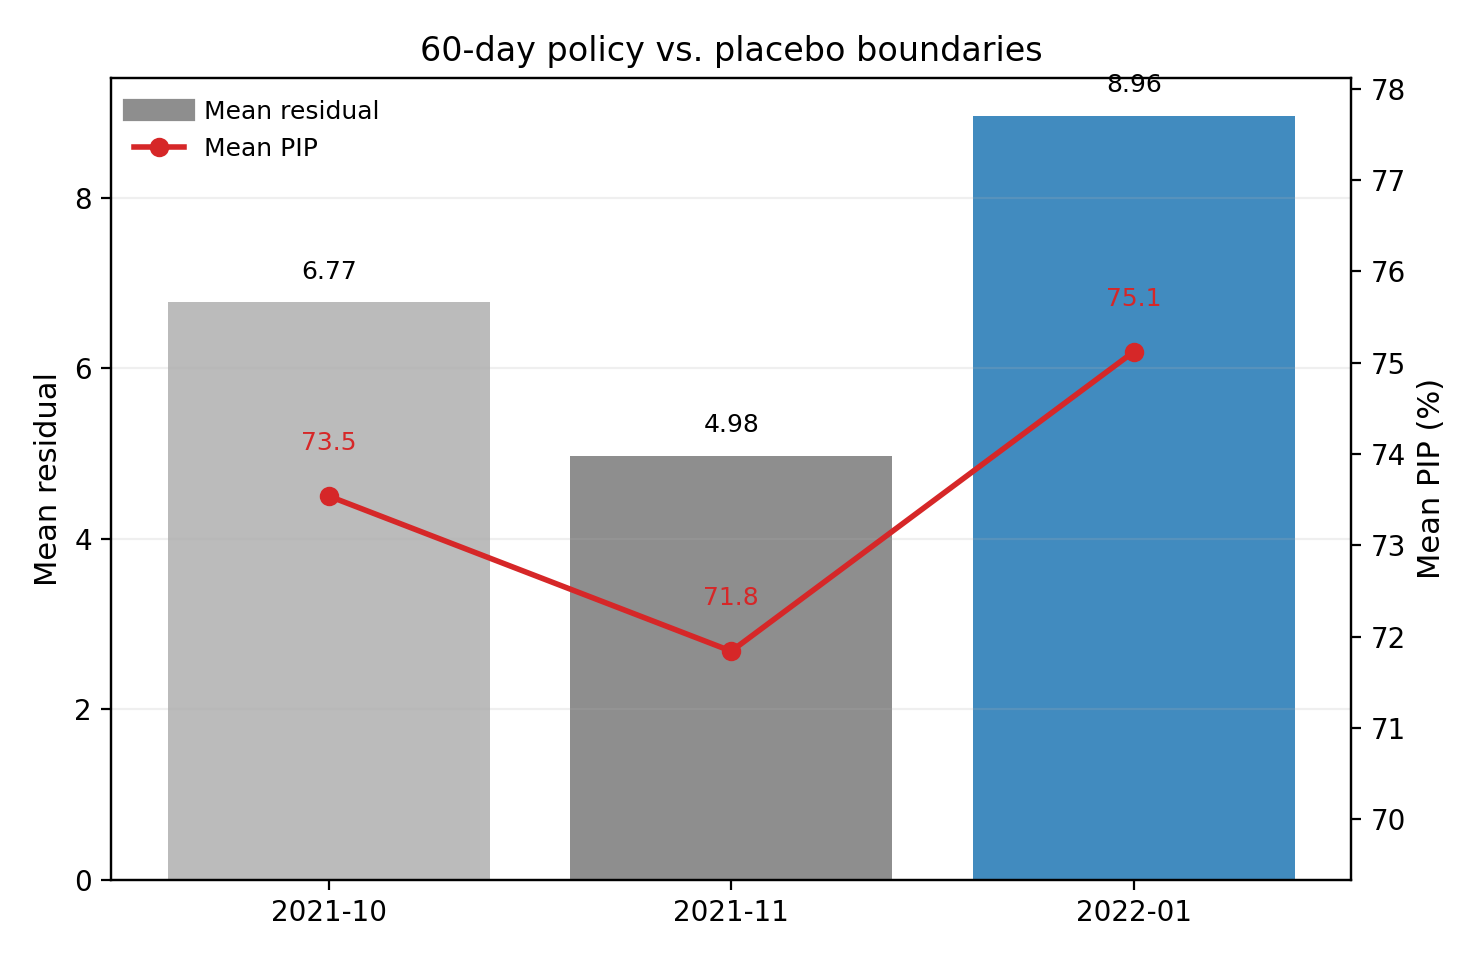
\includegraphics[width=.68\linewidth]{figures/placebo_boundary_comparison.png}
\caption{Fixed 60-day comparison between late-2021 placebo boundaries and the January 2022 policy boundary for the preferred LightGBM model with $w=6$.}
\label{fig:placebo}
\smallskip
\noindent\textit{Alt text: Bar chart comparing mean residual and mean PIP over the 60 days following October 2021, November 2021, and January 2022 boundaries. The January 2022 bars are the highest in both metrics.}
\end{figure}

\begin{figure}[htbp]
\centering
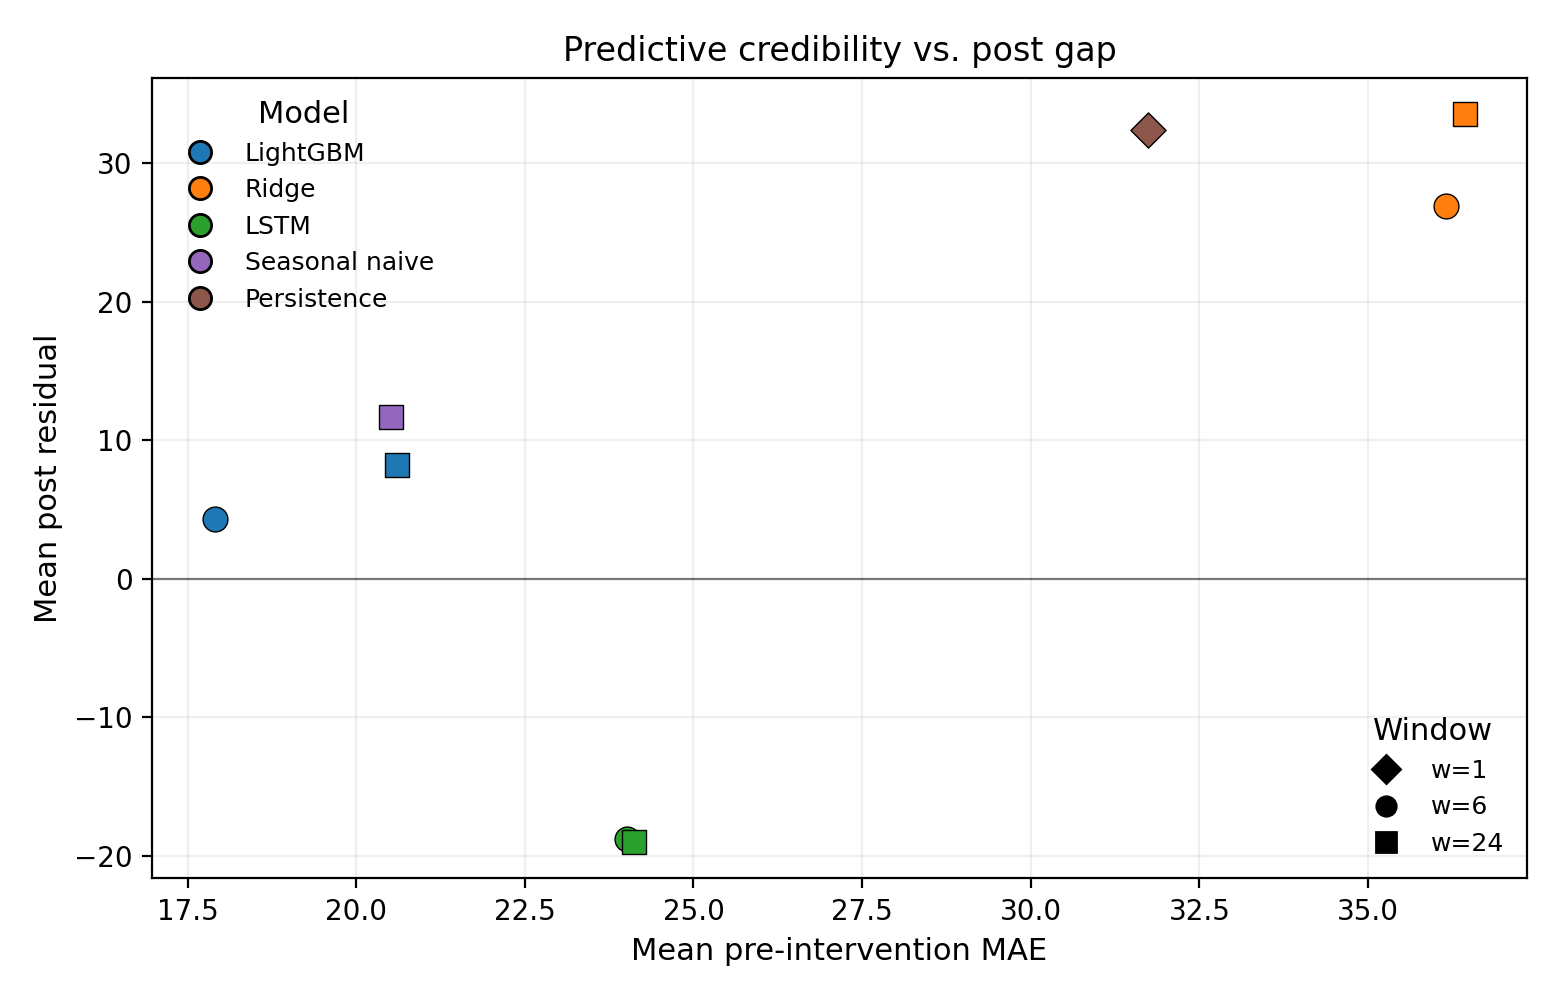
\includegraphics[width=.68\linewidth]{figures/credibility_tradeoff.png}
\caption{Relation between pre-policy MAE and mean post residual across learned models and naive baselines.}
\label{fig:tradeoff}
\smallskip
\noindent\textit{Alt text: Scatter plot of pre-policy MAE versus mean post residual, with colors for model family and marker shapes for window choice. LightGBM clusters in the lower-error region, while Ridge and persistence occupy higher-error regions with larger gaps.}
\end{figure}

\begin{figure}[htbp]
\centering
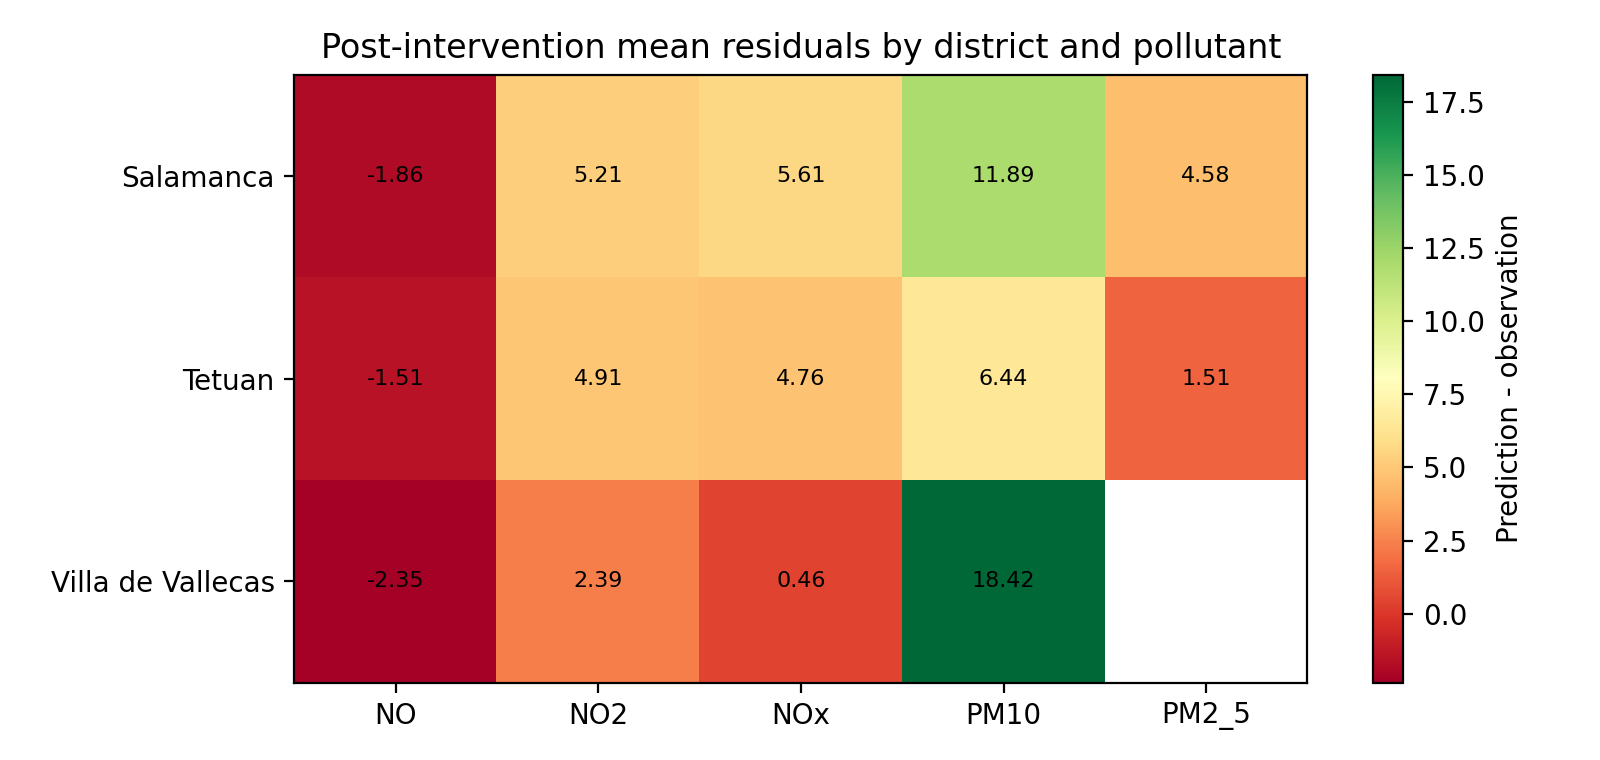
\includegraphics[width=.80\linewidth]{figures/best_full_variant_heatmap.png}
\caption{Post-policy mean residuals ($\hat{y} - y$) for the preferred full-feature LightGBM model with window $w=6$}
\label{fig:heatmap}
\smallskip
\noindent\textit{Alt text: Heatmap with districts on the vertical axis and pollutants on the horizontal axis. Most cells are positive, indicating observed pollution below the counterfactual forecast, with the strongest positive value for PM$_{10}$ in Villa de Vallecas and small negative NO residuals across the three districts.}
\end{figure}
